\chapter{Theoretical Framework}\label{chap:theoretical_framework}

\section{Introduction}\label{II-sec:introduction}

To formally represent geospatial knowledge in narratives, a comprehensive theoretical foundation is required, drawing on principles from narratology, geospatial data modeling, Semantic Web technologies, and ontology engineering. This chapter offers a detailed exploration of these foundational components, highlighting their significance in the context of geospatial narrative representation.

We begin with narratology, the study of how narratives are structured and conveyed. Tracing its roots to Aristotle’s Poetics and advancing through Russian Formalism, structuralism, and cognitive theories, narratology provides essential frameworks for understanding narrative structure. Key concepts include the distinction between \textit{fabula} (the chronological sequence of events) and \textit{syuzhet} (the narrative's presentation of those events). These concepts, along with the roles of characters and plots, are crucial for analyzing the dynamics of a narrative. Additionally, narratology offers insights into the differences between fictional narratives, which construct imagined worlds, and non-fictional narratives, grounded in real events.

Following this, we examine geospatial data modeling, beginning with the Feature-Based Approach and progressing through the Algebra and Calculi of Qualitative Spatial Relations, Topological Relations, Reasoning with Topological Relations, and Cardinal Directions. We also explore various representation techniques, such as Raster and Vector Representations, and Representation by Constraints, which are pivotal for accurately capturing spatial relationships in geospatial narratives.

Next, we introduce Semantic Web technologies, focusing on \acrshort{RDFLabel}, \acrshort{RDFSLabel}, \acrshort{OWLLabel}, and \acrshort{SPARQLLabel}. These technologies form the backbone for representing data, developing ontologies, and enabling sophisticated querying. They are integral to our research, providing the necessary infrastructure for semantic interoperability and data integration.

Finally, we turn to ontology engineering, outlining the methodologies and best practices for developing robust and interoperable ontologies. Emphasis is placed on methodological rigor, as well as the reuse of existing ontologies, to ensure efficiency and facilitate the seamless integration of diverse data sources. Through this approach, we ensure the creation of high-quality ontologies that support the formal representation of spatiotemporal narratives. 

\section{Introduction to Narratology}\label{II-sec:narratology}

Narratology is the study of narrative structures and the underlying logic, principles, and practices of their representation \cite{hermanBasicElementsNarrative2009}. Its origins trace back to Aristotle's Poetics, where narrative is described as the imitation of actions (\emph{praxis}) forming an argument (\emph{logos}), with events organized into a plot (\emph{mythos}) \cite{aristotelesPoetica2010}.

Later, Russian Formalism introduced the idea of a universal literary language or pattern of codes within a work's content, enabling narratives to be conveyed through various media like speech, writing, gestures, and music. Vladimir Propp's "Morphology of the Folktale" \cite{proppMorphologyFolktale1968} models folktales using 31 narrative functions and seven character roles or spheres of action.

Mid-20th-century structuralism further developed narratology. Claude Lévi-Strauss outlined a grammar of mythology, while A.~J.~Greimas proposed six fundamental narrative elements called \emph{actants} \cite{greimasStructuralSemanticsAttempt1983}. Tzvetan Todorov coins the term \emph{narratologie} \cite{todorovGrammaireDecameron1969}, and Gérard Genette analyzes narration separately from story content \cite{genetteNarrativeDiscourseEssay1990}.

Post-structuralist perspectives emerge in the 1980s \cite{fludernikHistoriesNarrativeTheory2005}, with Cognitive Narratology viewing narratology as a psychological phenomenon studied from a cognitive perspective \cite{davidhermanNarratologyCognitiveScience2000}. Cognitive psychology suggests that common-sense concepts often resist definition by necessary and sufficient conditions. While monotonic description logic captures aspects of conceptual knowledge, it falls short in representing prototypical knowledge; a general description logic for prototypical concepts remains undeveloped \cite{frixioneRepresentingConceptsFormal2012, lietoHybridRepresentationalProposal2014}.

\subsection{Fabula and Syuzhet}\label{II-subsec:fabulaAndSyzhet}

Russian Formalism distinguishes between \emph{fabula}, the chronological series of events at specific times and places, and \emph{syuzhet}, the author's presentation of these events \cite{proppMorphologyFolktale1968,lemonRussianFormalistCriticism1965}. Similarly, Chatman differentiates between \emph{story}, the content transmitted, and discourse, its particular organization \cite{chatmanCharactersNarratorsFilter1986}. Without a universal definition of narrative structure, some, like Crawford \cite{crawfordChrisCrawfordInteractive2012}, view narrative as a causality-based high-level structure independent of temporal or spatial relations. Genette identifies five key narrative concepts: order, frequency, duration, voice, and mood \cite{genetteNarrativeDiscourseEssay1990}. Bal adds a third level, presentation, the concrete representation of content delivered to the audience \cite{balNarratologyIntroductionTheory1997}.

\subsection{Characters and Plots}\label{II-subsec:charactersAndPlots}

Characters and plots are central to narratology. Characters, typically humans or humanoid beings, are fundamental to stories. While Aristotle emphasizes action \cite{aristotelesPoetica2010}, characters are indispensable in all tales. McKee argues that discussing plot without characters is impossible \cite{mckeeStorySubstanceStructure1997}. Chatman categorizes story elements into characters and setting elements like places and objects \cite{chatmanStoryDiscourseNarrative1978}. The plot consists of interconnected events forming a pattern within the story.

\subsection{Fictional vs. Non-fictional Narratives}\label{II-subsec:fictionalNonFictional}

A fundamental dichotomy in narratology is between fictional and non-fictional narratives \cite{jahnNarratology23Guide2021}. Fictional narratives aim to entertain and feature imaginary narrators and worlds, while Non-fictional narratives involve real-life narrators recounting actual events, such as news stories providing evidence of real occurrences.

\section{Geospatial Data Modeling}\label{II-sec:geospatialDataModeling}

This section discusses how to use mathematical abstractions to model the kinds of geospatial
information that we find in today’s applications. We consider only one way to modeling geospatial information, the feature based approach, because the field based approach is not usefult to the aim of this thesis. Then, we present three techniques for representing these abstract models in a computer: raster data, vector data, and constraints. The concept presented can also be explored in dept in Geospatial data science books, \cite{koubarakisGeospatialDataScience2023}, in \acrfull{GISLabel} books \cite{longleyGeographicInformationScience2015}, or books on geospatial DBMS \cite{rigauxSpatialDatabasesApplication2001, reveszIntroductionDatabasesBiological2010}.

\subsection{The Feature-Based Approach}\label{II-subsec:featureBased}


In \acrshort{GISLabel} terminology a geographic feature (or simply feature) is an abstraction of a real-world phenomenon and can have various attributes that describe its thematic and spatial characteristics \cite{longleyGeographicInformationScience2015}. For instance, features can represent the administrative divisions of a country, such as Italy. Thematic information about a specific administrative area, such as the municipality of Pisa, could include attributes like its name, population, and other socio-economic data. In contrast, spatial characteristics describe its geographical location and shape on Earth's surface.

Spatial attributes of a feature can be classified as either quantitative or qualitative. Quantitative spatial knowledge provides measurable data, such as distances. For example, the distance between Pisa and Florence is 90 kilometres. On the other hand, qualitative spatial knowledge refers to relational or descriptive information that cannot be easily quantified. For instance, the statement that the river Arno crosses Florence and Pisa and forms part of the border between Greece and Turkey is qualitative knowledge.

Quantitative geographic knowledge is generally represented using geometries, such as points, lines, and polygons \cite{rigauxSpatialDatabasesApplication2001, reveszIntroductionDatabasesBiological2010}. These geometries serve as abstractions of spatial features in the real world. Points can represent individual locations like cities, lines can depict rivers or roads, and polygons are used for larger areas such as administrative boundaries .

Qualitative geographic knowledge, however, is captured through qualitative binary relations between the geometries of features \cite{renzQualitativeSpatialReasoning2007}. These relations describe spatial interactions, such as adjacency or containment. For example, two polygons representing regions might share a common boundary (adjacency) or one region might be entirely contained within another .

Each geometry is associated with a \acrfull{CRSLabel}, which defines the coordinate space in which the geometry is embedded. A \acrshort{CRSLabel} uses one or more numbers, called coordinates, to uniquely specify the position of geometries within a particular space \cite{malingCoordinateSystemsMap1992}. In this thesis, we will consider Euclidean space as the coordinate system, where geometries are described and analyzed using familiar concepts from geometry and spatial mathematics.

The feature-based approach employs several classes of geometries, each suited to different types of spatial data. The geometries are displayed in figure \ref{fig:example_geometries} and can be categorized as follows::
\begin{enumerate}
    \item Point \\
    A point represents features whose shape is not of interest or that occupy an area much smaller than the space they are embedded in. Depending on the application, features like buildings, monuments, villages, or even cities can be modeled as points.

    \item Curve \\
    A curve is a one-dimensional geometry that connects points using different interpolation methods:

    \begin{itemize}
        \item Line String: A curve that uses linear interpolation between points. A line string is closed if its start and end points coincide, and simple if it has no self-intersections.
        \item Line: A line is a line string with exactly two points.
        \item Linear Ring: A line string that is both closed and simple.
    \end{itemize}

    \item Surface \\
    A surface is a two-dimensional geometry, typically represented by a single ``patch'' with one exterior boundary and zero or more interior boundaries (such as a polygon with holes). Types of surfaces include:
    
    \begin{itemize}
        \item Polygon: A simple planar surface with one exterior boundary and possibly several non-intersecting interior boundaries. It is topologically closed, and while boundaries may touch at a single point, they cannot intersect.
        \item Triangle: A specific type of polygon with three distinct, non-collinear vertices and no interior boundaries.
        \item Polyhedral Surface: A collection of polygons that share common boundary segments. Adjacent polygons share line segments, which are part of the boundary of at most two polygon patches.
        \item Triangulated Irregular Network (TIN): A polyhedral surface comprised exclusively of triangular patches.
    \end{itemize}
    
    \item Geometry Collection \\
    This is a set of distinct geometries, which can be further classified as follows:
    
    \begin{itemize}
        \item Multi-Point: A collection of points that are not connected.
        \item Multi-Curve: A collection of curves.
        \item Multi-Line String: A collection of line strings.
        \item Multi-Surface: A two-dimensional geometry collection consisting of surfaces. The geometric interiors of two surfaces may not overlap, and their boundaries may touch only at finite points.
        \item Multi-Polygon: A collection of polygons, where the boundaries of each polygon do not intersect.
    \end{itemize}

\end{enumerate}

\begin{figure}[h!tb]
    \centerline {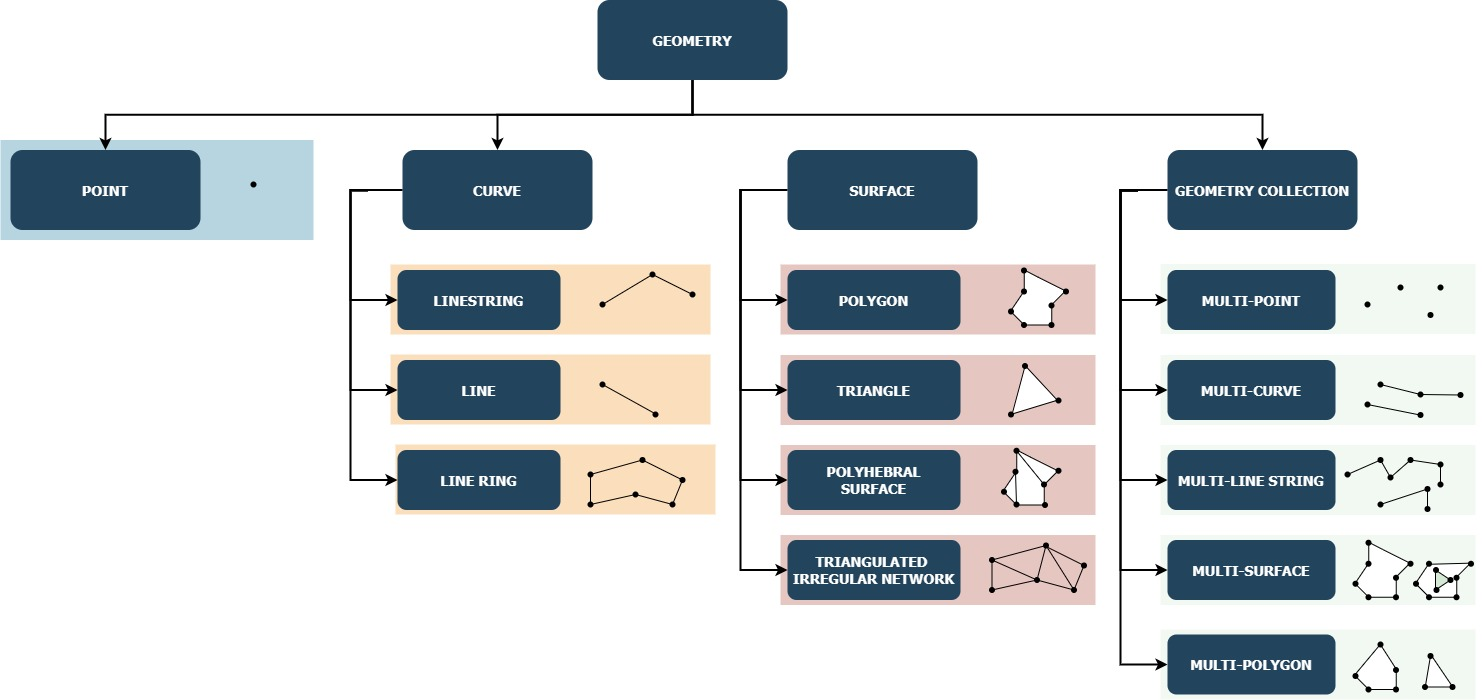
\includegraphics[width=\textwidth]{img/Geometries.jpg}}
    \caption{Classes of geometries in the feature-based model, exemplified by the geometry nearby.}
    \label{fig:example_geometries}
\end{figure}

\subsection{Algebra and Calculi of Qualitative Spatial Relations}\label{II-subsec:algebraCalculi}

Qualitative spatial relations provide a way to describe how spatial features relate to one another without relying on exact measurements. These relations are essential for capturing spatial knowledge in cases where precise quantitative data may not be available or necessary. Qualitative spatial relations can be categorized into various types, with topological relations being one of the most important.

Several algebras and calculi have been developed to formalize and reason about qualitative spatial relations. These formal systems define the rules and operations that can be applied to spatial relations to derive new information. Common calculi include the \acrfull{RCCLabel} and the 9-intersection model (9IM), both of which are widely used for reasoning with topological relations \cite{randellSpatialLogicBased1992}, \cite{egenhoferCategorizingBinaryTopological1991}. These frameworks enable efficient reasoning about how spatial features relate in terms of connectivity, adjacency, containment, and other qualitative properties.

% \paragraph{Region Connection Calculus (RCC)} The RCC is a formalism for representing and reasoning about spatial regions and their relationships. It defines several basic topological relations between regions, such as disconnection, external connection, partial overlap, and containment. This calculus allows for reasoning about how different spatial regions interact and relate to each other.

% \paragraph{9-Intersection Model} The 9-intersection model, proposed by Egenhofer, is another important formalism for spatial reasoning. It uses nine intersections between the boundaries, interiors, and exteriors of two spatial objects to classify their topological relations. The model identifies basic relations such as disjointness, overlap, and containment, among others.

\subsubsection{Topological Relations}\label{II-subsec:topologicalRelations}

Topology is a specialized field within mathematics that builds upon the foundations of geometry and set theory. It focuses on the study of spatial properties, such as space, dimension, and transformation, that remain unchanged under continuous deformation (stretching, twisting, etc.) \cite{janichTopology1984}. This approach is useful in geospatial systems where queries often include topological terms like "crosses" or "borders". For instance, questions such as "Which river crosses the city of Pisa?" or "Which municipalities border the municipality of Florence?" rely on understanding these spatial relationships.

Max Egenhofer made significant strides in this area by developing an algebra of binary topological relations that applied to two-dimensional regions with connected boundaries in ${\rm I\!R}^2$ \cite{egenhoferFormalDefinitionBinary1989}. His key contribution was the \acrfull{4IMLabel}, which categorizes topological relations based on the interactions of boundaries and interiors between two regions. In the 4IM, the classification of relationships is based on the intersections of the boundaries and interiors of two features $A_1$, $A_2$. Each intersection may be empty $(0)$ or nonempty $(\neg 0)$, resulting in a total of $2^4 = 16$ combinations. Each case is represented by a matrix of values:

\begin{equation}
M = 
\begin{pmatrix} 
\partial A_1 \cap \partial A_2 & \partial A_1 \cap A_2^{\circ} \\ 
A_1^{\circ} \cap \partial A_2 & A_1^{\circ} \cap A_2^{\circ} 
\end{pmatrix}
\end{equation}

The interior $A^{\circ}$ of a generic feature $A$ may be defined as:

\begin{equation}
A^{\circ} = A - \partial A,
\end{equation}

where $\partial A$ denotes the boundary of $A$.

Considerating the area/area cases there are 8 possible relationship: disjoint, meet, contains, covers, equal, overlap, inside, and coveredBy showed in figure \ref{fig:4IM}

\begin{figure}[h!tb]
    \centerline {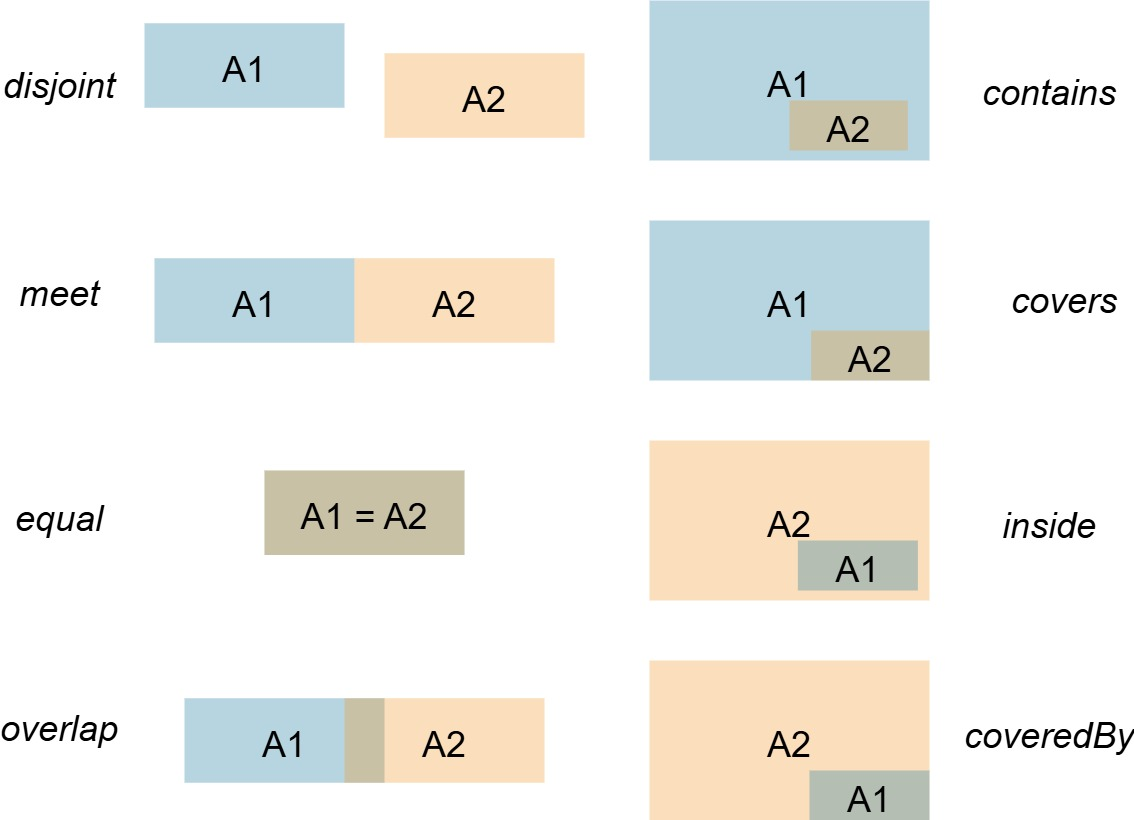
\includegraphics[width=\textwidth]{img/4IM.jpg}}
    \caption{The eight relations area/area of 4IM.}
    \label{fig:4IM}
\end{figure}

Building on the \acrshort{4IMLabel}, Egenhofer and Herring extended this model by incorporating the exterior of the regions, leading to the development of the \acrfull{9IMLabel} \cite{egenhoferCategorizingBinaryTopological1991}. While \acrshort{9IMLabel} provides the same region-to-region relations as the \acrshort{4IMLabel}, it expands the framework to include more detailed interactions between regions, lines, and points, generating a total of 56 \acrshort{JEPDLabel} relations. The \acrshort{9IMLabel} also considers the exterior of features, besides interior and boundary. The exterior $A^{-}$ of a feature $A$ is defined as:

\begin{equation}
A^{-} = \mathbb{R}^2 - A,
\end{equation}

Therefore, it is necessary to consider the following matrix of nine sets:

\begin{equation}
M = 
\begin{pmatrix} 
\partial A_1 \cap \partial A_2 & \partial A_1 \cap A_2^{\circ}  & \partial A_1 \cap A_2^{-} \\ 
A_1^{\circ} \cap \partial A_2 & A_1^{\circ}  \cap A_2^{\circ}  & A_1^{\circ}  \cap A_2^{-} \\
A_1^{-} \cap \partial A_2 & A_1^{-} \cap A_2^{\circ}  & A_1^{-} \cap A_2^{-} 
\end{pmatrix}
\end{equation}


Later, Clementini and his colleagues introduced further enhancements by considering the dimension of each intersection, which resulted in the \acrfull{DE9IMLabel} \cite{clementiniSmallSetFormal1993, clementiniComparisonMethodsRepresenting1995a}. The \acrshort{DE9IMLabel} provides a more nuanced approach by accounting for up to 81 \acrshort{JEPDLabel} binary topological relations. This model uses a 3x3 matrix, where each cell represents the dimensional relationship between different parts of two regions—such as their boundaries, interiors, and exteriors. The matrix's values reflect whether these intersections are empty, of a specific dimension, or simply irrelevant.

The \acrshort{DE9IMLabel} accounts for 81 \acrshort{JEPDLabel} binary topological relations. If we denote  $dim(A)$ the dimension the following 3 × 3 matrix M gives us all these 81 binary topological relations between regions A1 and A2:

\begin{equation}
M = 
\begin{pmatrix} 
dim(\partial A_1 \cap \partial A_2) & dim(\partial A_1 \cap A_2^{\circ}) & dim(\partial A_1 \cap A_2^{-}) \\ 
dim(A_1^{\circ} \cap \partial A_2) & dim(A_1^{\circ}  \cap A_2^{\circ}) & dim(A_1^{\circ} \cap A_2^{-}) \\
dim(A_1^{-} \cap \partial A_2) & dim(A_1^{-} \cap A_2^{\circ}) & dim(A_1^{-} \cap A_2^{-})
\end{pmatrix}
\end{equation}

The cells of \( M \) can take the following values: \( -1 \) (empty intersection), \( 0, 1, 2, T \) (true) = \(\{0, 1, 2\}\), \( F \) (false) = \(\{-1\}\), and \( * \) (don’t care) = \(\{-1, 0, 1, 2\}\).


In parallel, Tony Cohn and his team at the University of Leeds developed the \acrfull{RCCLabel}, which provides another way to describe the spatial relationships between regions \cite{randellSpatialLogicBased1992}. \acrshort{RCCLabel} is centered around the concept of "is connected to" binary predicate. There is a very close correspondence between the relations of 4IM, DE9IM, and RCC-8 captured in table \ref{tab:comparingRCC8_4IM_DE9IM}. However, \acrshort{9IMLabel} and \acrshort{DE9IMLabel} only consider single-piece regions without holes in two-dimensional space while RCC-8 allows much more general regions. This makes reasoning in \acrshort{9IMLabel} and \acrshort{DE9IMLabel} harder than reasoning in \acrshort{RCCLabel} \cite{grigniTopologicalInference1995, renzCanonicalModelRegion2002}.
    

\begin{table}[h!tb]
   \centering \caption{Comparing 4IM, RCC-8, and DE9IM}
   \label{tab:comparingRCC8_4IM_DE9IM}
   \vskip 0.2cm
   %%
   \scalebox{0.90}{
	    %% The {|c|c|c|c|c|} define the number of columns.
	    %% c means centered
	    %% | defines a vertical line between two columns 
	    \begin{tabular}{|c|c|c|}
	      \hline
	      \textbf{4IM} & \textbf{RCC-8} & \textbf{DE9IM}  \\
            \hline
            \textit{equals} & EQ & \textit{equals} \\
            \hline
            \textit{disjoint} & DC & \textit{disjoint} \\
            \hline
            \textit{intersects} & $\neg$ DC & $\neg$ \textit{disjoint} \\
            \hline
            \textit{touches} & EC & \textit{meet} \\
            \hline
	        \textit{within} & (NTPP, TPP) & \textit{(inside, coveredBy)} \\
            \hline
            \textit{contains} & (NTPP-1, TPP-1) & \textit{contains,covers} \\
            \hline
            \textit{overlaps} & PO & \textit{overlap} \\
	      \hline
	      
	    \end{tabular}
	 }
 \end{table}

One challenge in dealing with topological relations is the uncertainty in determining the exact relationship between regions. In such cases, disjunctive expressions, which combine several possible relations, are used to describe what is known. For example, the relationship between two regions A and B might be expressed as a disjunction like $A \left( PO \lor TPP \lor NTPP \right) B$, capturing the possibility of multiple topological configurations.

In some cases, RCC-5, a simplified version of RCC-8, is used. RCC-5 ignores the boundary of regions, thus reducing the number of distinct relations by combining some of the RCC-8 relations. For instance, it merges distinctions like "disconnected" (DC) and "externally connected" (EC) into a single "discrete from" (DR) relation, and simplifies "proper part" (TPP and NTPP) into a single "proper part" (PP) relation.

% \subsubsection{Reasoning with Topological Relations}

% The field of qualitative spatial reasoning and related research in geographic information systems (GIS) and spatial databases has produced a wealth of insights on how to reason using topological relations. Reviews by Cohn and Renz [2008], as well as Renz and Nebel [2007], provide comprehensive overviews of the progress in this area.

% One major problem in this field is determining the consistency of a set of topological statements. For example, given regions A, B, and C, consider the following RCC-8 relations: A is a tangential proper part of B (ANTPPB), B is a tangential proper part of C (BNTPPC), and C is disconnected from A (CDCA). These statements are inconsistent because the relationships between the regions cannot simultaneously hold. Consistency-checking algorithms rely on constraint networks [Dechter 2003, Rossi et al. 2006], which represent spatial relations as constraints between pairs of regions. In an RCC-8 constraint network, nodes represent regions, and edges represent possibly disjunctive relations between them. Techniques like path consistency and efficient backtracking are often employed to resolve these disjunctions [Renz and Nebel 2007].

% Reasoning with disjunctive relations (i.e., where the exact relation is unknown but multiple possibilities are specified) is NP-hard, but research has identified certain tractable subsets of RCC-8 relations [Renz and Nebel 2007]. For example, if the network contains only basic RCC-8 relations (no disjunctions), the consistency problem can be solved in polynomial time using path consistency algorithms [Renz and Nebel 1999]. Unfortunately, the same is not true for DE9IM, where the corresponding problem remains NP-hard [Grigni et al. 1995].

% Another important reasoning task is computing entailments—deriving new relationships based on existing ones. For example, if A is a tangential proper part of B (ANTPPB) and B is a tangential proper part of C (BNTPPC), we can infer that A is a tangential proper part of C (ANTPPC). This is usually done using transitivity tables and constraint propagation methods. Table 2.2 provides an example of such a transitivity table for RCC-8 relations.

% \subsubsection{Cardinal directions} 
% Cardinal direction form another important aspect of qualitative spatial relations. These relations describe how objects are positioned relative to one another using directions like north, south, east, and west. Cardinal direction relations are particularly useful in applications such as navigation, geographic information systems, and spatial querying, where relative orientation is important.

% Cardinal direction relations can be formalized using frameworks such as the \textit{Cardinal Direction Calculus} (CDC) \cite{frank1991}. This calculus captures the relative positions of spatial objects based on the principal directions (north, south, east, west) and often includes intermediate directions (e.g., northeast, southwest). In such a model, a relation between two regions might be expressed as follows: "Region \(A\) is north of Region \(B\)" or "Region \(C\) is to the southeast of Region \(D\)".

% CDC-based reasoning can be applied in spatial databases and GIS for tasks such as retrieving objects located in a particular direction from a reference point or for aligning spatial data based on relative positions. For example, in urban planning, cardinal direction reasoning can be used to plan developments with respect to existing infrastructure, ensuring that new projects are positioned according to specific directional requirements.


\subsection{Representation Techniques}\label{II-subsec:representationTechniques}

The representation of spatial data is a critical aspect \acrshort{GISLabel} and spatial reasoning. Different techniques can be employed depending on the nature of the data and the required level of precision. The most common representation techniques include raster representation, vector representation, and representation by constraints. Each method has its advantages and limitations, depending on the application and type of spatial data.

\subsubsection{Raster Representation}\label{II-subsubsec:raster}
Raster representation uses a grid of equally spaced cells or pixels to represent spatial information. Each cell in the raster grid holds a value that represents some property of the space at that location, such as elevation, temperature, or land cover. Raster data is particularly useful for representing continuous spatial phenomena, such as terrain or satellite imagery.

The resolution of a raster dataset depends on the size of the cells; smaller cells provide higher resolution but require more storage space. This representation is ideal for applications that require the analysis of spatial patterns or gradual changes across a landscape. However, it may not be the most efficient for representing discrete features, such as roads or administrative boundaries, where vector data may be more appropriate \cite{burroughPrinciplesGeographicalInformation1986}.

\subsubsection{Vector Representation}\label{II-subsubsec:vector}
In contrast, vector representation uses geometric shapes—points, lines, and polygons—to represent spatial features. Points can represent discrete locations, such as cities or landmarks, lines are used for linear features like rivers or roads, and polygons represent areas such as administrative boundaries or land parcels.

Vector data is ideal for representing discrete, well-defined features with precise boundaries. It is often preferred in applications that require detailed spatial analysis or where the exact shape and position of features are important. The storage of vector data is generally more efficient than raster data for discrete features, and vector models are widely used in \acrshort{GISLabel} for tasks such as map-making, spatial querying, and network analysis \cite{goodchildGeographicalDataModeling1992}.

\subsubsection{Representation by Constraints}\label{II-subsubsec:constraint}
Representation by constraints is a more abstract method for representing spatial features. Rather than explicitly storing the shape or geometry of a feature, this technique represents spatial objects through a set of constraints or rules that must be satisfied. These constraints may describe spatial relationships, such as proximity, containment, or alignment, between features.

This representation is particularly useful in scenarios where spatial data is incomplete, uncertain, or imprecise. By specifying constraints, it is possible to define the relationships between features without requiring precise geometrical data. This method is often employed in qualitative spatial reasoning, where the goal is to reason about the relationships between spatial objects rather than their exact locations or shapes \cite{clarkeSituationalCrimePrevention1997}.

\subsubsection{Comparison of Representation Techniques}\label{II-subsubsec:comparisonRepresentation}

Each representation technique has its strengths and weaknesses, depending on the nature of the spatial data and the specific application. Raster representation is well-suited for continuous data and large-scale spatial patterns, but it can be inefficient for representing discrete features. Vector representation is highly efficient for discrete features with precise boundaries, but it may not perform as well when dealing with continuous phenomena. Representation by constraints is ideal for reasoning about spatial relationships in the absence of precise data, but it may require more computational effort to derive specific geometric properties.


\section{Semantic Web Technologies}\label{II-sec:semantic_web_technologies}

The Semantic Web extends the current web by enabling sharing and reusing data across applications, enterprises, and communities. It relies on formal knowledge representation to structure data in a machine-readable and interoperable format \cite{berners-leeSemanticWebNew2001}. This section provides a detailed overview of Semantic Web technologies foundational to this research. We explain how the \acrshort{RDFLabel} models data as triples, how the \acrshort{OWLLabel} facilitates complex ontology definitions, and how \acrshort{SPARQLLabel} enables querying of \acrshort{RDFLabel} data.

\subsection{ \acrfull{RDFLabel}}\label{II-subsec:rdf}

The \acrlong{RDFLabel} is a standard model for data interchange on the web \cite{beckettDesignImplementationRedland2002, danbrickleyRDFSchema112014, mcbrideResourceDescriptionFramework2004}. The \acrshort{RDFLabel} framework facilitates the representation of information about resources in graph form. It operates on the principle of articulating statements about resources through subject-predicate-object expressions, commonly referred to as triples. An \acrshort{RDFLabel} triple comprises a subject, the resource being described, a predicate, the property or aspect of the subject, and an object, which can be either another resource or a literal value representing the property's value.

For example, the statement "Sherlock Holmes is an enemy of Dr. Moriarty" can be represented as:

\begin{itemize}
    \item Subject: \texttt{ex:sherlock}
    \item Predicate: \texttt{ex:isEnemyOf}
    \item Object: \texttt{ex:moriarty}
\end{itemize}

This triple can be visualized as a directed graph, where nodes represent resources and edges represent predicates.

\subsubsection{\acrfull{TurtleLabel}}\label{II-subsubsec:turtle}

\acrfull{TurtleLabel} is one of the most common syntaxes for expressing \acrshort{RDFLabel} data. It is a compact, human-readable format that is closely related to \acrshort{SPARQLLabel}, an \acrshort{RDFLabel} query language. Although \acrshort{RDFLabel} can be serialized in various formats, such as \textit{N-Triples}, \textit{JSON-LD}, and \textit{RDF/XML}, \acrshort{TurtleLabel} is preferred in this thesis for its simplicity and readability.

For example, in Turtle, the previous \acrshort{RDFLabel} triple could be written as:
\begin{lstlisting}[caption=Example triple in Turtle with prefixed names, label={lst:prefix-names}]
    ex:sherlock ex:isEnemyOf ex:moriarty
\end{lstlisting}

This concise representation helps developers work with \acrshort{RDFLabel} data more efficiently, especially when dealing with large datasets.

\subsubsection{\acrfullpl{IRILabel}}\label{II-subsubsec:iri}

\acrshort{RDFLabel} uses \acrfullpl{IRILabel} to uniquely identify resources. \acrshortpl{IRILabel} ensure that each resource is globally unique, facilitating data integration from multiple sources. An \acrshort{IRILabel} is a string of characters used to identify resources uniquely. It is an extension of the \acrfull{URILabel}, allowing the inclusion of non-ASCII characters, making it more adaptable to a globalized web. \acrshortpl{IRILabel} can be represented in three primary forms in Turtle:

\begin{itemize}
    \item Absolute \acrshort{IRILabel} represents a complete \acrshort{IRILabel} \\
    \texttt{<http://example.org/sherlock>}.
    \item Relative \acrshort{IRILabel} is a shorter version that refers to a base \acrshort{IRILabel} \\
    \texttt{<sherlock>}.
    \item Prefixed Names combines a prefix and a local name \\
    \texttt{ex:sherlock}. The prefix (e.g., \texttt{ex:}) is defined in the \acrshort{TurtleLabel} document.
\end{itemize}

\subsubsection{Literals and Data Types}\label{II-subsubsec:literals}

Objects in \acrshort{RDFLabel} triples can be literals, which are concrete values such as strings, numbers, or dates. Literals can have data types specified using XML Schema data types \cite{paulv.bironXMLSchemaPart2004}. For instance:

\begin{lstlisting}[caption=Example triple in Turtle with an integer literal, label={lst:integer-literal}]
ex:Paris ex:population "2148327"^^xsd:integer .
\end{lstlisting}

\subsection{\acrfull{RDFSLabel}}\label{II-subsec:rdfs}

\acrfull{RDFSLabel} extends \acrshort{RDFLabel} by providing a basic vocabulary for describing properties and classes of  \acrshort{RDFLabel} resources \cite{danbrickleyRDFSchema112014}. Key elements in \acrshort{RDFSLabel} include Classes, defined using \texttt{rdfs:Class} to represent groups of resources, and Properties, defined using \texttt{rdfs:Propery} to represent relationships between resources. Subclass relationships are specified using \texttt{rdfs:subClassOf}, which establishes class hierarchies. Additionally, Domain and Range are specified using \texttt{rdfs:domain} and \texttt{rdfs:range}, indicating the classes to which a property applies and the type of values it can have.


\subsection{\acrfull{OWLLabel}}\label{II-subsec:owl}

The acrfull{OWLLabel} is designed for representing rich and complex knowledge about things, groups of things, and relations between things \cite{OWLWebOntologya,bechhoferOWLWebOntology2009, OWLWebOntologyb, OWLWebOntologyc}. \acrshort{OWLLabel} builds upon \acrshort{RDFLabel} and \acrshort{RDFSLabel}, offering greater expressiveness for defining ontologies.

The World Wide Web Consortium (W3C) classifies \acrshort{OWLLabel} into three sub languages: \acrshort{OWLLabel} Lite, \acrshort{OWLLabel} DL, and \acrshort{OWLLabel} Full \cite{bechhoferOWLWebOntology2009}.

\begin{itemize}
    \item \acrshort{OWLLabel} Lite is the simplest version of \acrshort{OWLLabel}, providing a basic classification hierarchy and simple constraints. It permits only the expression of relationships with a maximum cardinality of 0 or 1, making it easier to implement. \acrshort{OWLLabel} Lite restricts \acrshort{OWLLabel} DL to a subset of language constructors and lacks certain features such as explicit negation and union. The main disadvantage of \acrshort{OWLLabel} Lite is its limited expressiveness due to these restrictions.
    \item \acrshort{OWLLabel} DL is named for its foundation in Description Logic, a formalism used to represent the relationships between objects and their properties. It offers maximum expressiveness while preserving computational completeness and decidability. This means that any reasoning task will always terminate and provide a correct result. Decidability was a core design criterion for \acrshort{OWLLabel} DL, and many syntactic restrictions are imposed to guarantee this property.
    \item \acrshort{OWLLabel} Full provides the highest level of expressiveness and the syntactic freedom of \acrshort{RDFLabel} but without guarantees on computational complexity. In \acrshort{OWLLabel} Full, computational aspects were not a primary consideration in its design—only logical and semantic aspects were emphasized. Since it does not introduce the syntactic restrictions that \acrshort{OWLLabel} DL uses to retain decidability, reasoning over \acrshort{OWLLabel} Full ontologies can be undecidable, meaning that a reasoner may not always terminate or return a correct result.
\end{itemize}

\subsubsection{Classes, Properties, and Individuals}\label{II-subsubsec:classesProperties}

\acrshort{OWLLabel} allows the definition of three fundamental components: Classes, Properties, and Individuals. Classes represent sets of individuals and serve as categories or types within the ontology. Properties define relationships either between individuals or between individuals and data values, effectively connecting different parts of the ontology. Individuals are the instances of classes, representing the actual objects or entities within the domain of discourse.

\subsubsection{Complex Class Expressions}\label{II-subsubsec:classExpression}

\acrshort{OWLLabel} supports complex class expressions using logical operators such as Intersection, Union, and Complement. The Intersection operator (\texttt{owl
}) defines a class as the intersection of multiple classes, meaning an individual must belong to all specified classes to be a member of this new class. The Union operator (\texttt{owl
}) defines a class as the union of multiple classes, so an individual belonging to any of the specified classes is considered a member of the union class. The Complement operator (\texttt{owl
}) defines a class as the complement of another class, encompassing all individuals that are not members of the specified class.

\subsubsection{Property Characteristics}\label{II-subsubsec:properyCharachteristics}

\acrshort{OWLLabel} allows properties to have specific characteristics, including being Transitive, Symmetric, or Functional. A Transitive property implies that if individual \texttt{A} is related to individual \texttt{B} through this property, and \texttt{B} is related to \texttt{C}, then \texttt{A} is also related to \texttt{C}. A Symmetric property means that if \texttt{A} is related to \texttt{B}, then \texttt{B} is necessarily related to \texttt{A} through the same property. A Functional property is one where each individual can have at most one value for that property, ensuring that the property maps individuals to a single unique value.

\subsubsection{Reasoning and Inference}\label{II-subsubsec:reasoning}

\acrshort{OWLLabel}'s formal semantics enable automated reasoning using description logic reasoners like Pellet \cite{sirinPelletPracticalOWLDL2007}. These reasoners can perform tasks such as Consistency Checking, which involves verifying that the ontology does not contain contradictory information, ensuring logical coherence. They can also perform Classification, determining subclass relationships and organizing the ontology's hierarchy based on defined criteria. Additionally, reasoners handle Instance Checking, determining whether a particular individual is an instance of a specific class by evaluating the individual's properties and relationships against class definitions.

\subsection{\acrfull{SPARQLLabel}}\label{II-subsec:sparql}

\acrshort{SPARQLLabel} plays a pivotal role in querying and manipulating \acrshort{RDFLabel} graphs by using pattern matching techniques \cite{ericprudhommeauxSPARQLQueryLanguage2008}. It enables users to efficiently retrieve, manipulate, and transform data stored in \acrshort{RDFLabel} format, providing powerful capabilities for interacting with structured data on the web.

A typical \acrshort{SPARQLLabel} query comprises several essential components:

\begin{itemize}
    \item \texttt{PREFIX} declarations: These are used to define namespace abbreviations, simplifying the use of long \acrshortpl{URILabel} within the query and making it more readable.
    \item \texttt{SELECT} clause: Specifies the variables to return as part of the query results.
    \item \texttt{WHERE} clause: Contains a set of triple patterns that the query processor matches against the \acrshort{RDFLabel} dataset.
    \item \texttt{FILTER} clause: Applies additional constraints on variables, offering precise control over the query output.
\end{itemize}

Here is an example query that retrieves all cities and their respective populations:

\begin{lstlisting}[caption=Example SPARQL query that retrieves all cities and their population, label={lst:sparql-example}]
PREFIX ex: <http://example.org/> 
SELECT ?city ?population 
WHERE { 
  ?city rdf:type ex:City . 
  ?city ex:hasPopulation ?population . 
} 
\end{lstlisting}

\acrshort{SPARQLLabel} provides a wide range of advanced features to enable more sophisticated data retrieval and analysis:

\begin{itemize}
    \item \textbf{Optional Patterns}: The \texttt{OPTIONAL} keyword is used to include data in the query results if available, without causing the query to fail if that data is missing. This is useful when dealing with incomplete data.
    \item \textbf{Union}: The \texttt{UNION} keyword allows the query to combine multiple patterns, retrieving data that matches any of the specified conditions.
    \item \textbf{Aggregations}: Functions like \texttt{COUNT}, \texttt{SUM}, and \texttt{AVG} are available to perform calculations on the query results, enabling direct data aggregation and analysis within the query itself.
    \item \textbf{Subqueries}: Subqueries allow nesting of queries inside a larger query, breaking down complex data retrieval into manageable components and supporting multi-step data analysis.
\end{itemize}

\subsubsection{\acrshort{SPARQLLabel} Endpoints and Remote Data Access}\label{II-subsubsec:SPARQL}

\acrshort{SPARQLLabel} endpoints serve as interfaces that allow querying \acrshort{RDFLabel} data over the web. These endpoints accept \acrshort{SPARQLLabel} queries via HTTP requests and return results in various formats such as XML, JSON, or CSV. By supporting remote access to \acrshort{RDFLabel} datasets, \acrshort{SPARQLLabel} endpoints facilitate seamless integration of distributed data sources, enabling applications and users to query and analyze data across the web.


\subsection{Data Sharing and Interoperability}\label{II-subsec:data_sharing}

Semantic Web technologies are pivotal for advancing data sharing and interoperability across diverse systems. By adhering to standardized formats, leveraging linked data principles, and reusing established vocabularies, these technologies enable seamless integration of heterogeneous data sources.

\subsubsection{Standardization}\label{II-subsubsec:standardization}

Interoperability is driven by the adoption of universally recognized standards and protocols. The Technologies introduced in the previous sections, such as \acrshort{RDFLabel} \ref{II-subsec:rdf}, \acrshort{OWLLabel} \ref{II-subsec:owl}, and \acrshort{SPARQLLabel} \ref{II-subsec:sparql} provide the necessary structure for consistent data representation and querying across systems. These standards ensure that data can be interpreted and exchanged uniformly, regardless of the system architecture or implementation.

\subsubsection{Linked Data Principles}\label{II-subsubsec:lod}

Tim Berners-Lee’s principles of Linked Data propose a framework for publishing structured data on the web, emphasizing interlinking to create a global data space \cite{timberners-leeLinkedDataDesign2006}. By following these principles, data published on the web can be made accessible, interrelated, and actionable by both humans and machines. This approach fosters a web of interconnected data, enriching information discovery and facilitating broader data integration.

\subsubsection{Vocabulary Reuse}\label{II-subsubsec:vocabularyReuse}

The reuse of existing ontologies and standardized vocabularies is crucial for ensuring semantic consistency and minimizing redundancy. In the forthcoming chapters, we will present a collection of vocabularies and ontologies for reuse. Leveraging these established frameworks improves system compatibility and aligns semantic interpretations.

% \section{Ontology Engineering}\label{sec:ontology_engineering}

% Ontology engineering is the systematic methodology for designing and constructing ontologies, essential for defining shared vocabularies in specific domains. This process emphasizes methodological rigor, efficient reuse of existing ontologies, and the enhancement of both interoperability and operational efficiency. Below, we outline the key stages involved in the ontology development lifecycle, followed by strategies for ontology reuse and a set of best practices.

% \subsection{Ontology Development Lifecycle}

% Ontology development typically progresses through a series of structured stages, each focusing on different aspects of ontology creation and refinement \cite{fernandez-lopezMETHONTOLOGYOntologicalArt1997}:

% \subsubsection{Specification}

% The specification phase defines the ontology's purpose, scope, and requirements. It involves identifying the domain, the intended use cases, and the competency questions that the ontology is expected to address. This stage is critical in ensuring that the ontology is designed with a clear focus and is aligned with the needs of its users.

% \subsubsection{Conceptualization}

% In the conceptualization stage, domain knowledge is organized into a structured format by identifying key concepts, relationships, and constraints. Conceptual models such as taxonomies or class diagrams are often developed at this stage, providing a blueprint for the ontology’s structure.

% \subsubsection{Formalization}

% The formalization stage involves translating the conceptual model into a formal, machine-readable representation using ontology languages such as OWL. This formal representation enables logical inference and automated reasoning, ensuring that the ontology can be computationally processed and interpreted.

% \subsubsection{Implementation}

% Once formalized, the ontology is implemented using tools such as Protégé \cite{musenProtegeProject2015}. This stage involves encoding the ontology’s classes, properties, instances, and axioms. During implementation, the conceptual and formal models are transformed into an operational ontology that can be deployed and queried.

% \subsubsection{Evaluation}

% Evaluation is a critical phase where the ontology is assessed for its correctness, completeness, and consistency. Evaluation methods include validation against the original competency questions and logical consistency checks, often using automated reasoners. Ensuring that the ontology meets the required standards of quality is essential for its effectiveness in real-world applications.

% \subsubsection{Maintenance}

% As the domain evolves, the ontology must be updated to remain relevant. The maintenance phase ensures that the ontology reflects current knowledge, adapts to new requirements, and continues to meet user needs over time. Ongoing refinement and updates are essential to maintain the ontology's accuracy and utility.

% \subsection{Reuse of Existing Ontologies}

% Reusing existing ontologies is a best practice in ontology engineering, as it accelerates development, enhances interoperability, and ensures alignment with established standards. The primary strategies for ontology reuse include:

% \begin{itemize} \item \textbf{Importing}: Incorporating entire ontologies or specific modules from existing ones to leverage their predefined structures and relationships. \item \textbf{Aligning}: Mapping concepts between different ontologies to establish equivalences or hierarchies, facilitating data integration across diverse domains. \item \textbf{Extending}: Enhancing existing ontologies by adding new concepts, properties, or relationships to meet additional requirements while retaining compatibility with established ontologies. \end{itemize}

% \subsection{Best Practices in Ontology Engineering}

% Adopting best practices in ontology engineering ensures the creation of robust, maintainable, and reusable ontologies. Key best practices include:

% \begin{itemize} \item \textbf{Modularity}: Designing ontologies as modular components to enhance reusability, maintainability, and scalability. Modular ontologies allow for easier updates and integration with other ontologies. \item \textbf{Documentation}: Providing comprehensive and clear documentation of the ontology’s structure, purpose, and design decisions. Good documentation is crucial for enabling others to understand, use, and extend the ontology. \item \textbf{Versioning}: Implementing a version control system to manage changes over time, track modifications, and ensure backward compatibility. This practice supports transparency and allows for incremental improvements. \item \textbf{Community Engagement}: Involving domain experts and stakeholders in the development process. Collaborative engagement ensures the ontology reflects expert knowledge and meets community needs, increasing its adoption and relevance. \end{itemize}


\section{Conclusion}\label{II-sec:conclusion}

This chapter laid the theoretical foundation essential for representing geospatial knowledge within narrative structures, integrating principles from narratology, geospatial data modeling, Semantic Web technologies, and ontology engineering. Each of these areas contributes critical tools for the formalization and interpretation of spatiotemporal narratives, facilitating the structured representation of complex geospatial phenomena.

The exploration of narratology provided key insights into the structure and dynamics of narratives, distinguishing between the chronological sequence of events (\textit{fabula}) and their narrative presentation (\textit{syuzhet}). These distinctions are pivotal for understanding both fictional and non-fictional narratives, enabling a nuanced approach to narrative analysis in geospatial contexts. The significance of characters, plots, and narrative structure also emphasized the necessity of defining clear roles and causal relationships within geospatial stories.

Geospatial data modeling, with its focus on the feature-based approach, qualitative spatial relations, and topological reasoning, offered the mathematical and logical tools needed to capture and model spatial relationships within narratives. This approach, combined with effective data representation techniques such as raster and vector models, provides a flexible and precise framework for encoding spatial features in narrative contexts.

Semantic Web technologies, including \acrshort{RDFLabel}, \acrshort{OWLLabel}, and \acrshort{SPARQLLabel}, demonstrated their critical role in enabling interoperability, data integration, and semantic querying, forming the backbone of the formal systems that support geospatial narrative representation. The ability to link data and ensure semantic coherence across multiple domains is crucial for building comprehensive and interoperable geospatial systems.

Finally, the principles of ontology engineering highlighted the importance of methodological rigor, reuse of existing ontologies, and best practices in creating robust, scalable, and maintainable ontologies. This ensures that the formal representation of geospatial narratives is both semantically rich and operationally efficient, allowing for seamless data integration and reasoning across diverse systems.

Together, these theoretical components form a cohesive framework that supports the formal representation and analysis of geospatial narratives, laying the groundwork for further exploration and practical applications in subsequent chapters.

Chapter \ref{chap:overview_narratives} examines the crucial elements of geospatial, spatiotemporal, and narrative representations, providing a detailed overview of the interplay between these domains to facilitate formalized representations of intricate knowledge. Through the exploration of fundamental ontologies pertinent to each field, the pivotal importance of interoperability and reuse is underscored, fostering the seamless integration of data and improved reasoning across various systems.
